\documentclass[envcountsect,dvips]{beamer}

\setbeamertemplate{background canvas}[vertical shading][bottom=yellow!20,top=blue!10]
%\usetheme{Darmstadt}
\usetheme{Warsaw}
%\usefonttheme[onlysmall]{structurebold}

\usepackage{natbib}
\usepackage{bibentry}
\bibliographystyle{plain}
\usepackage{chngcntr}

\usepackage[utf8]{inputenc}
\usepackage{default}
\usepackage{amsmath}
\usepackage{amsfonts}
\usepackage{amssymb}

\usepackage{graphicx}
\usepackage{caption}
\usepackage{subcaption}

\usepackage{color,xcolor,ucs}% para textcolor



\newenvironment<>{varblock}[2][.9\textwidth]{%
  \setlength{\textwidth}{#1}
  \begin{actionenv}#3%
    \def\insertblocktitle{#2}%
    \par%
    \usebeamertemplate{block begin}}
  {\par%
    \usebeamertemplate{block end}%
  \end{actionenv}}

%%%%%%%%%%%%%%%%%%%%%%%%%%%%%%%%%%%%%%%%%%%%%%%%%%%%%%%%%%%%%%%%%%%%%%%%%%
\begin{document}

\title[Hierarquia de memoria:   ] % (optional, only for long titles)
{Hierarquia da memoria:}
\subtitle{Capacidade, velocidade e custo}
\author[Fernando] % (optional, for multiple authors)
{Fernando Pujaico Rivera\inst{1}}
\institute[Universidade Federal de Lavras] % (optional)
{
  \inst{1}%
  Universidade Federal de Lavras
}
\date[2016] % (optional)
{Aula-1 2016}
\subject{Computer Science}
\frame{\titlepage}

%%%%%%%%%%%%%%%%%%%%%%%%%%%%%%%%%%%%%%%%%%%%%%%%%%%%%%%%%%%%%%%%%%%%%%%%%%%%%%%%
%%%%%%%%%%%%%%%%%%%%%%%%%%%%%%%%%%%%%%%%%%%%%%%%%%%%%%%%%%%%%%%%%%%%%%%%%%%%%%%%
%%%%%%%%%%%%%%%%%%%%%%%%%%%%%%%%%%%%%%%%%%%%%%%%%%%%%%%%%%%%%%%%%%%%%%%%%%%%%%%%
\section{Hierarquia da memoria}

%%%%%%%%%%%%%%%%%%%%%%%%%%%%%%%%%%%%%%%%%%%%%%%%%%%%%%%%%%%%%%%%%%%%%%%%%%%%%%%%%
\begin{frame}{Objetivo\cite{arq}}
Objetivos ao construir um sistema de memoria de um computador:
\begin{block}{Alta capacidade}
Bytes, KB, MB, GB, TB
\end{block}
\begin{block}{Alta velocidade}
bits/seg, Kbps, Mbps
\end{block}
\begin{block}{Baixo custo}
Dólares por byte
\end{block}
\end{frame}


%%%%%%%%%%%%%%%%%%%%%%%%%%%%%%%%%%%%%%%%%%%%%%%%%%%%%%%%%%%%%%%%%%%%%%%%%%%%%%%%%
\begin{frame}{Objetivo\cite{arq}}
\begin{minipage}[c]{0.5\textwidth}
\begin{varblock}{Estrutura piramidal}
Misturar memorias:
\begin{description}
 \item[pequenas, rápidas e custosas:] 
 Dados com maior probabilidade de aceso.
 \item[grandes lentas e baratas:] 
 Dados com menor probabilidade de aceso.
\end{description}
\end{varblock}
\end{minipage}%
\begin{minipage}[c]{0.5\textwidth}
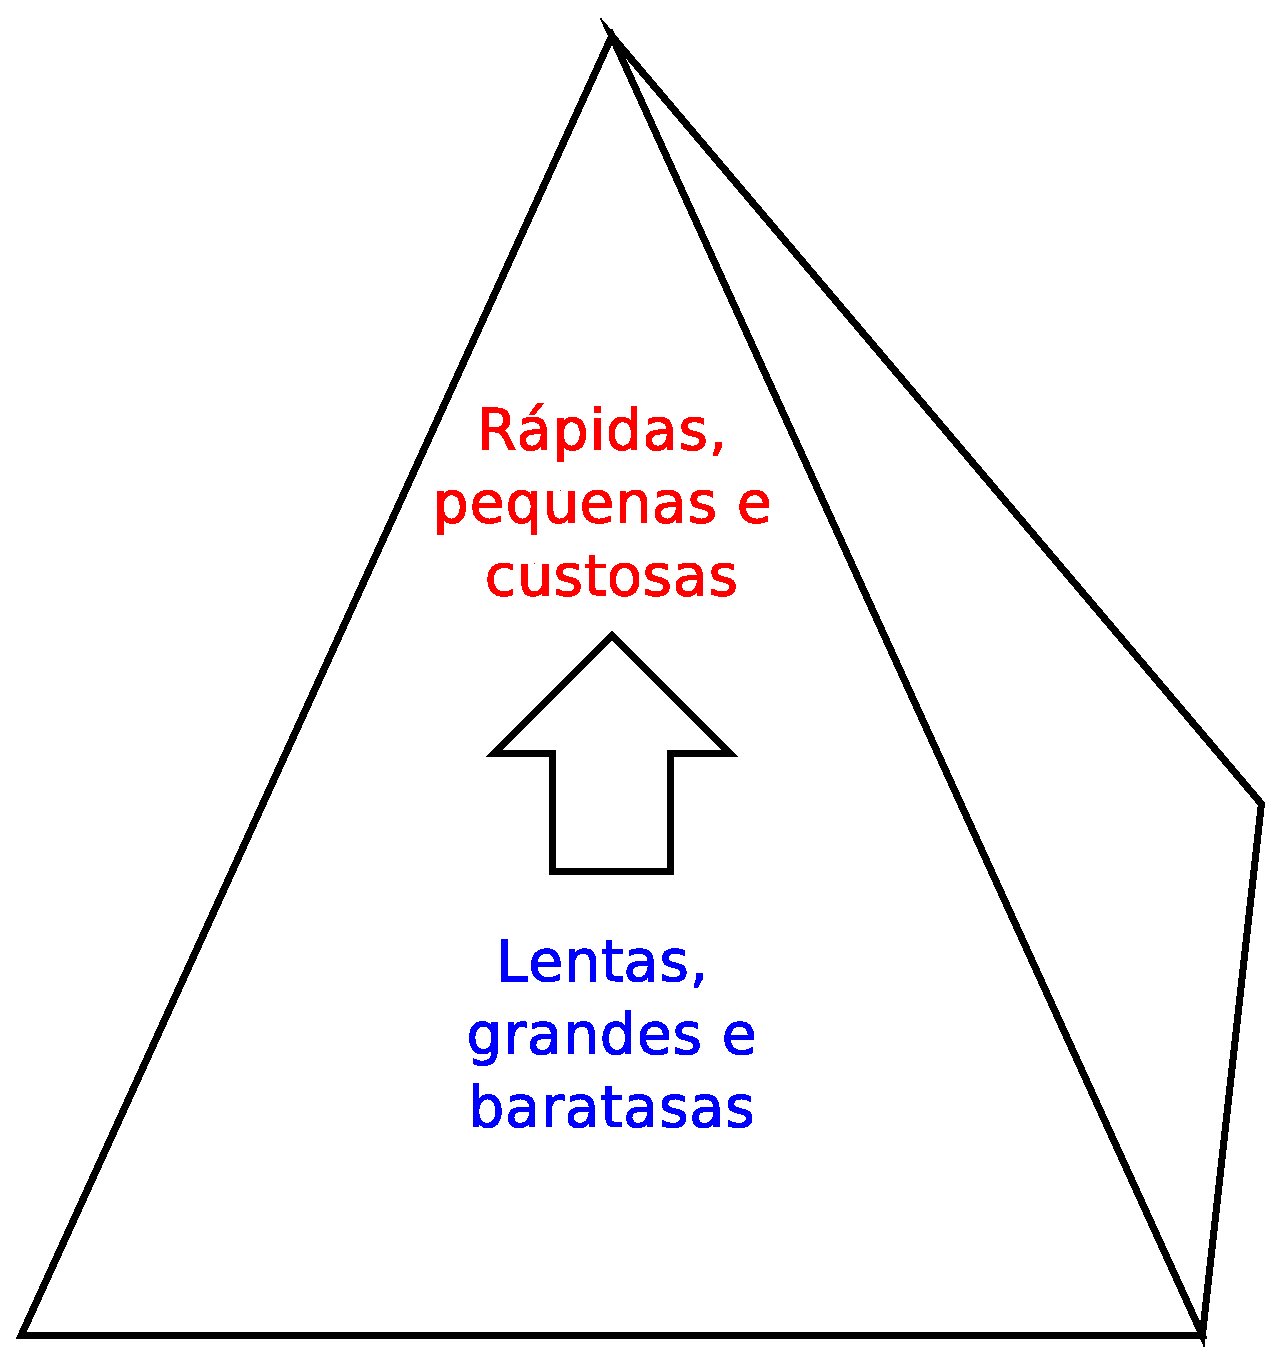
\includegraphics[width=0.8\textwidth]{images/piramidal.eps}
\end{minipage}
\end{frame}

%%%%%%%%%%%%%%%%%%%%%%%%%%%%%%%%%%%%%%%%%%%%%%%%%%%%%%%%%%%%%%%%%%%%%%%%%%%%%%%%%
\begin{frame}{Principio de localidade}
Conhecer a probabilidade de uso - Principio de localidade
\begin{minipage}[c]{0.5\textwidth}
\begin{varblock}{Principio de \\localidade espacial}
Meu vizinho e eu
\end{varblock}
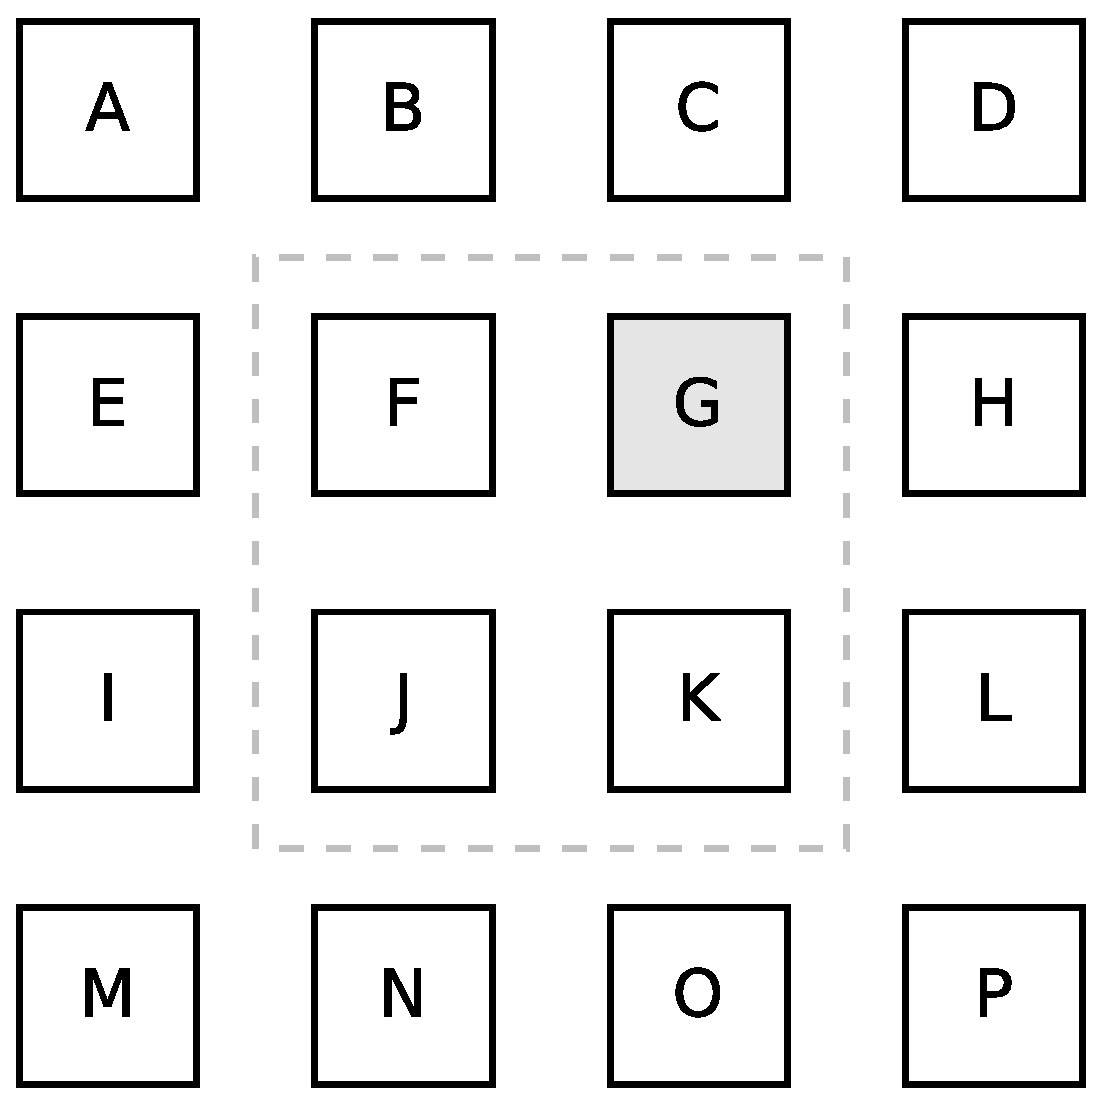
\includegraphics[width=0.8\textwidth]{images/lespacial.eps}
\end{minipage}%
\begin{minipage}[c]{0.5\textwidth}
\begin{varblock}{Principio de \\localidade temporal}
Você me verá de novo
\end{varblock}
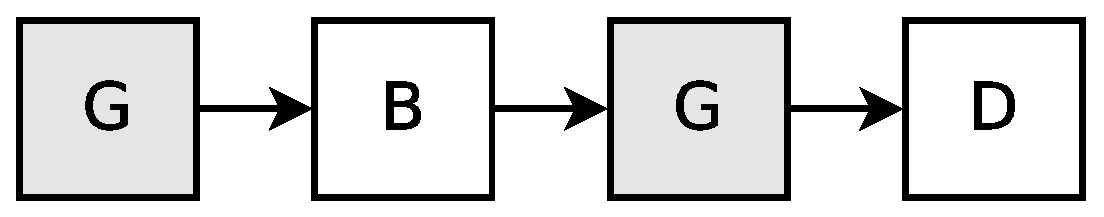
\includegraphics[width=0.9\textwidth]{images/ltemporal.eps}
~\\
~\\
~\\
~\\
~\\
~\\
~\\
\end{minipage}
\end{frame}

%%%%%%%%%%%%%%%%%%%%%%%%%%%%%%%%%%%%%%%%%%%%%%%%%%%%%%%%%%%%%%%%%%%%%%%%%%%%%%%%%
%%%%%%%%%%%%%%%%%%%%%%%%%%%%%%%%%%%%%%%%%%%%%%%%%%%%%%%%%%%%%%%%%%%%%%%%%%%%%%%%%
\section{Níveis da hierarquia}

%%%%%%%%%%%%%%%%%%%%%%%%%%%%%%%%%%%%%%%%%%%%%%%%%%%%%%%%%%%%%%%%%%%%%%%%%%%%%%%%%
\begin{frame}{Níveis da hierarquia de memoria}
\begin{center}
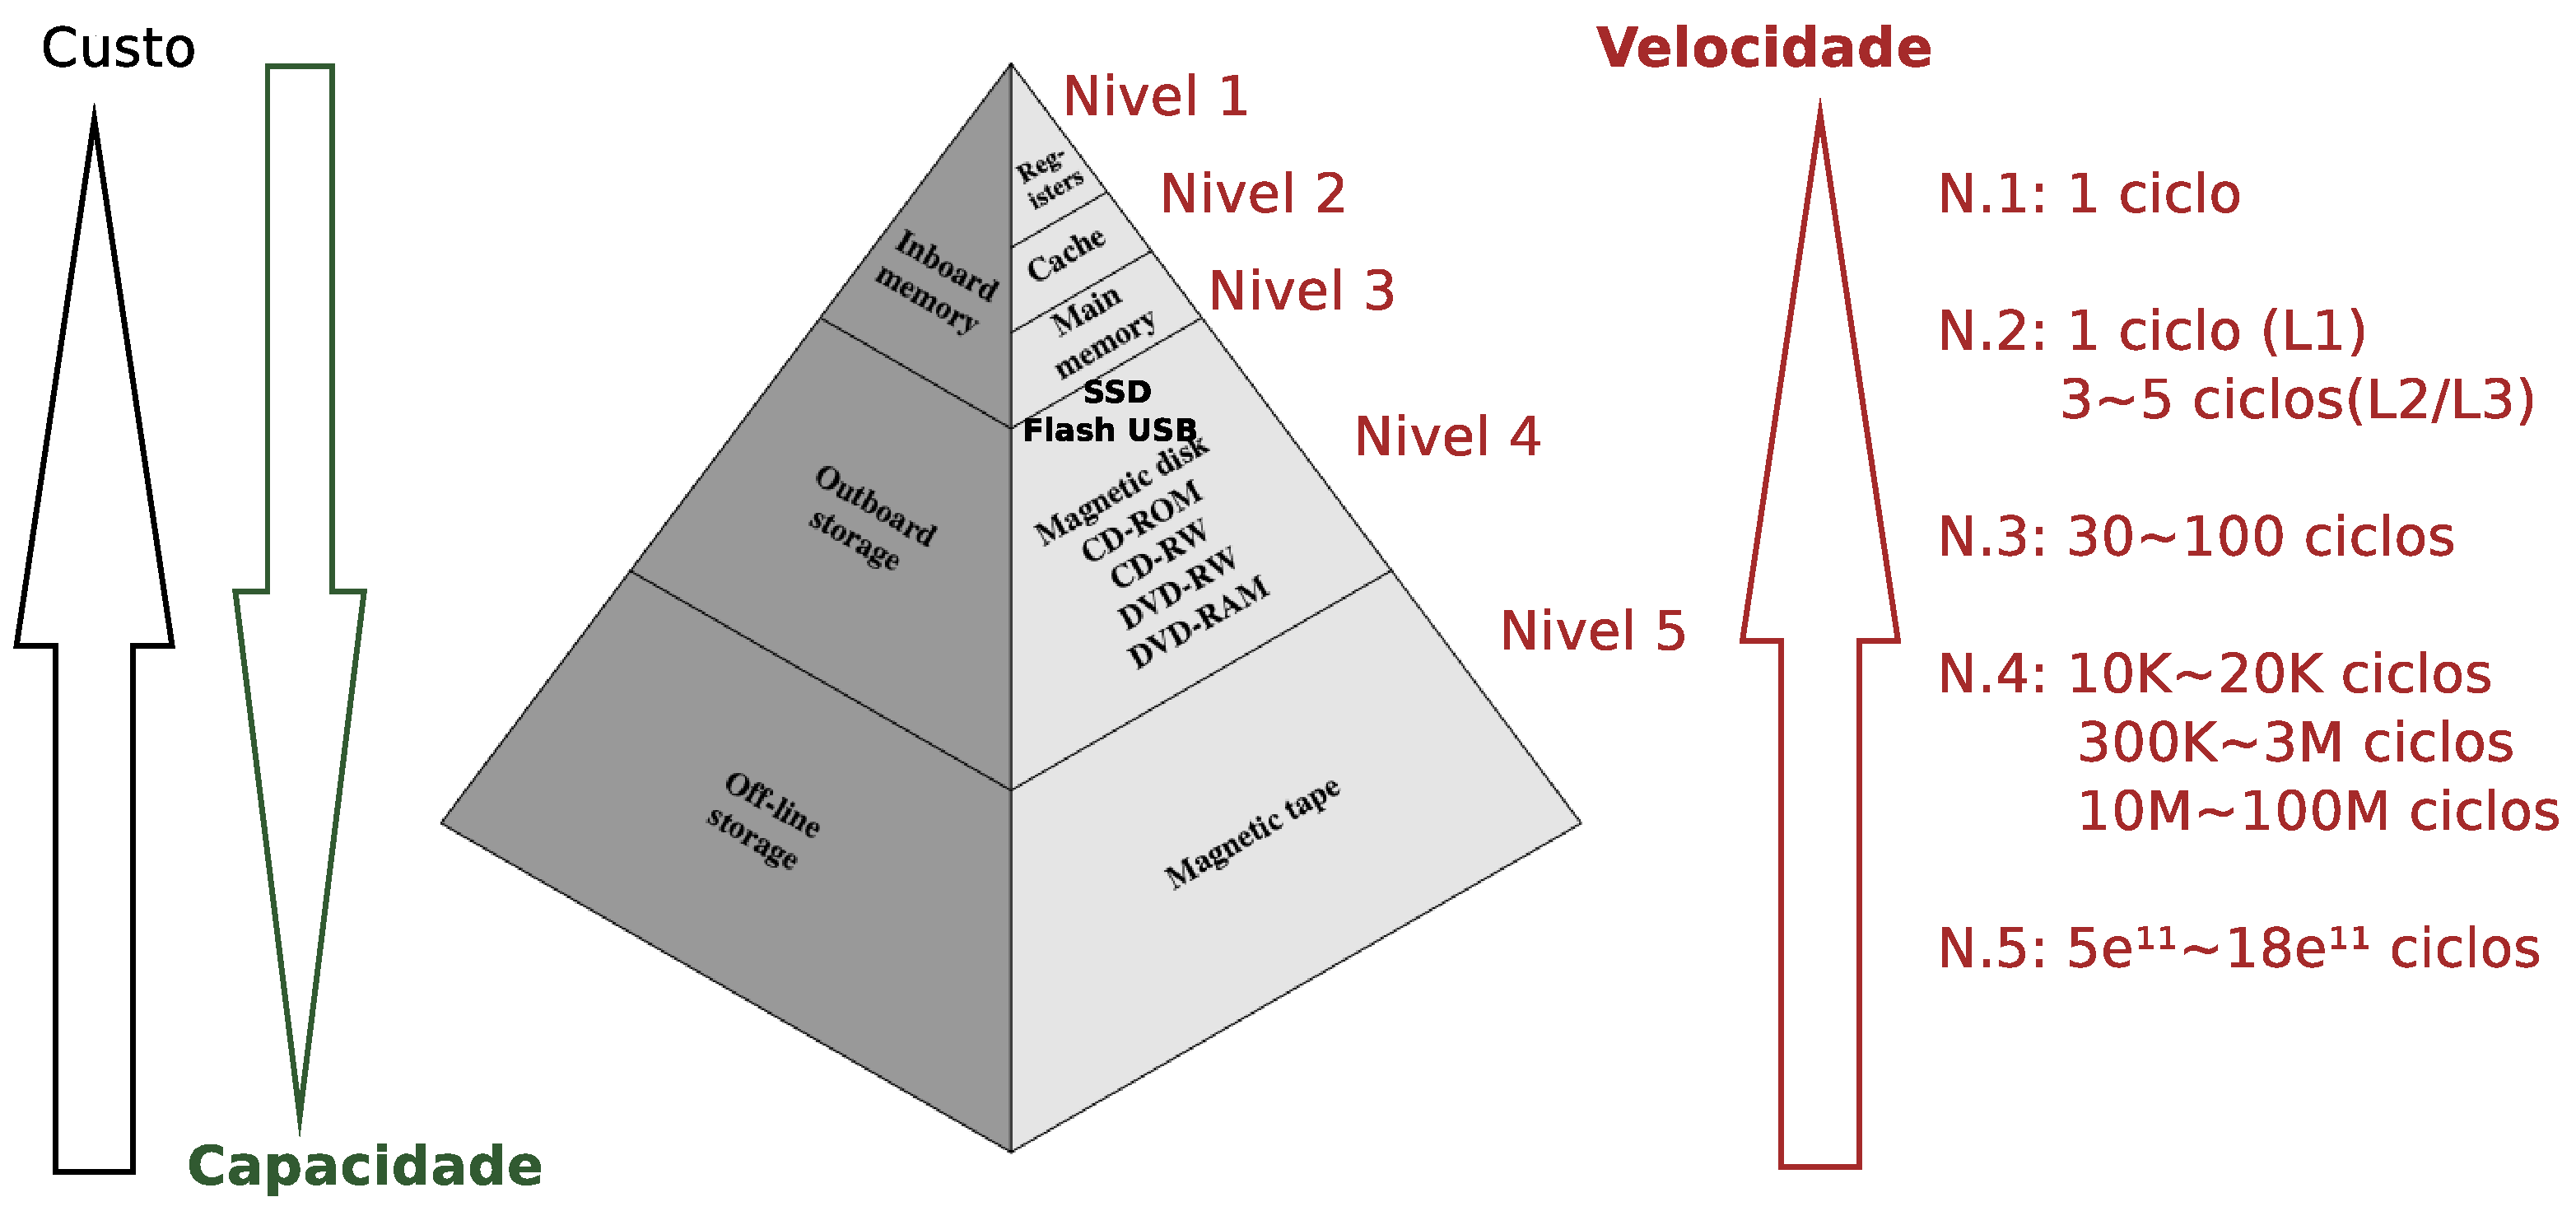
\includegraphics[width=1.0\textwidth]{images/piramidal2.eps}
\end{center}
\end{frame}
%%%%%%%%%%%%%%%%%%%%%%%%%%%%%%%%%%%%%%%%%%%%%%%%%%%%%%%%%%%%%%%%%%%%%%%%%%%%%%%%%
\begin{frame}{Níveis da hierarquia de memoria}
\begin{center}
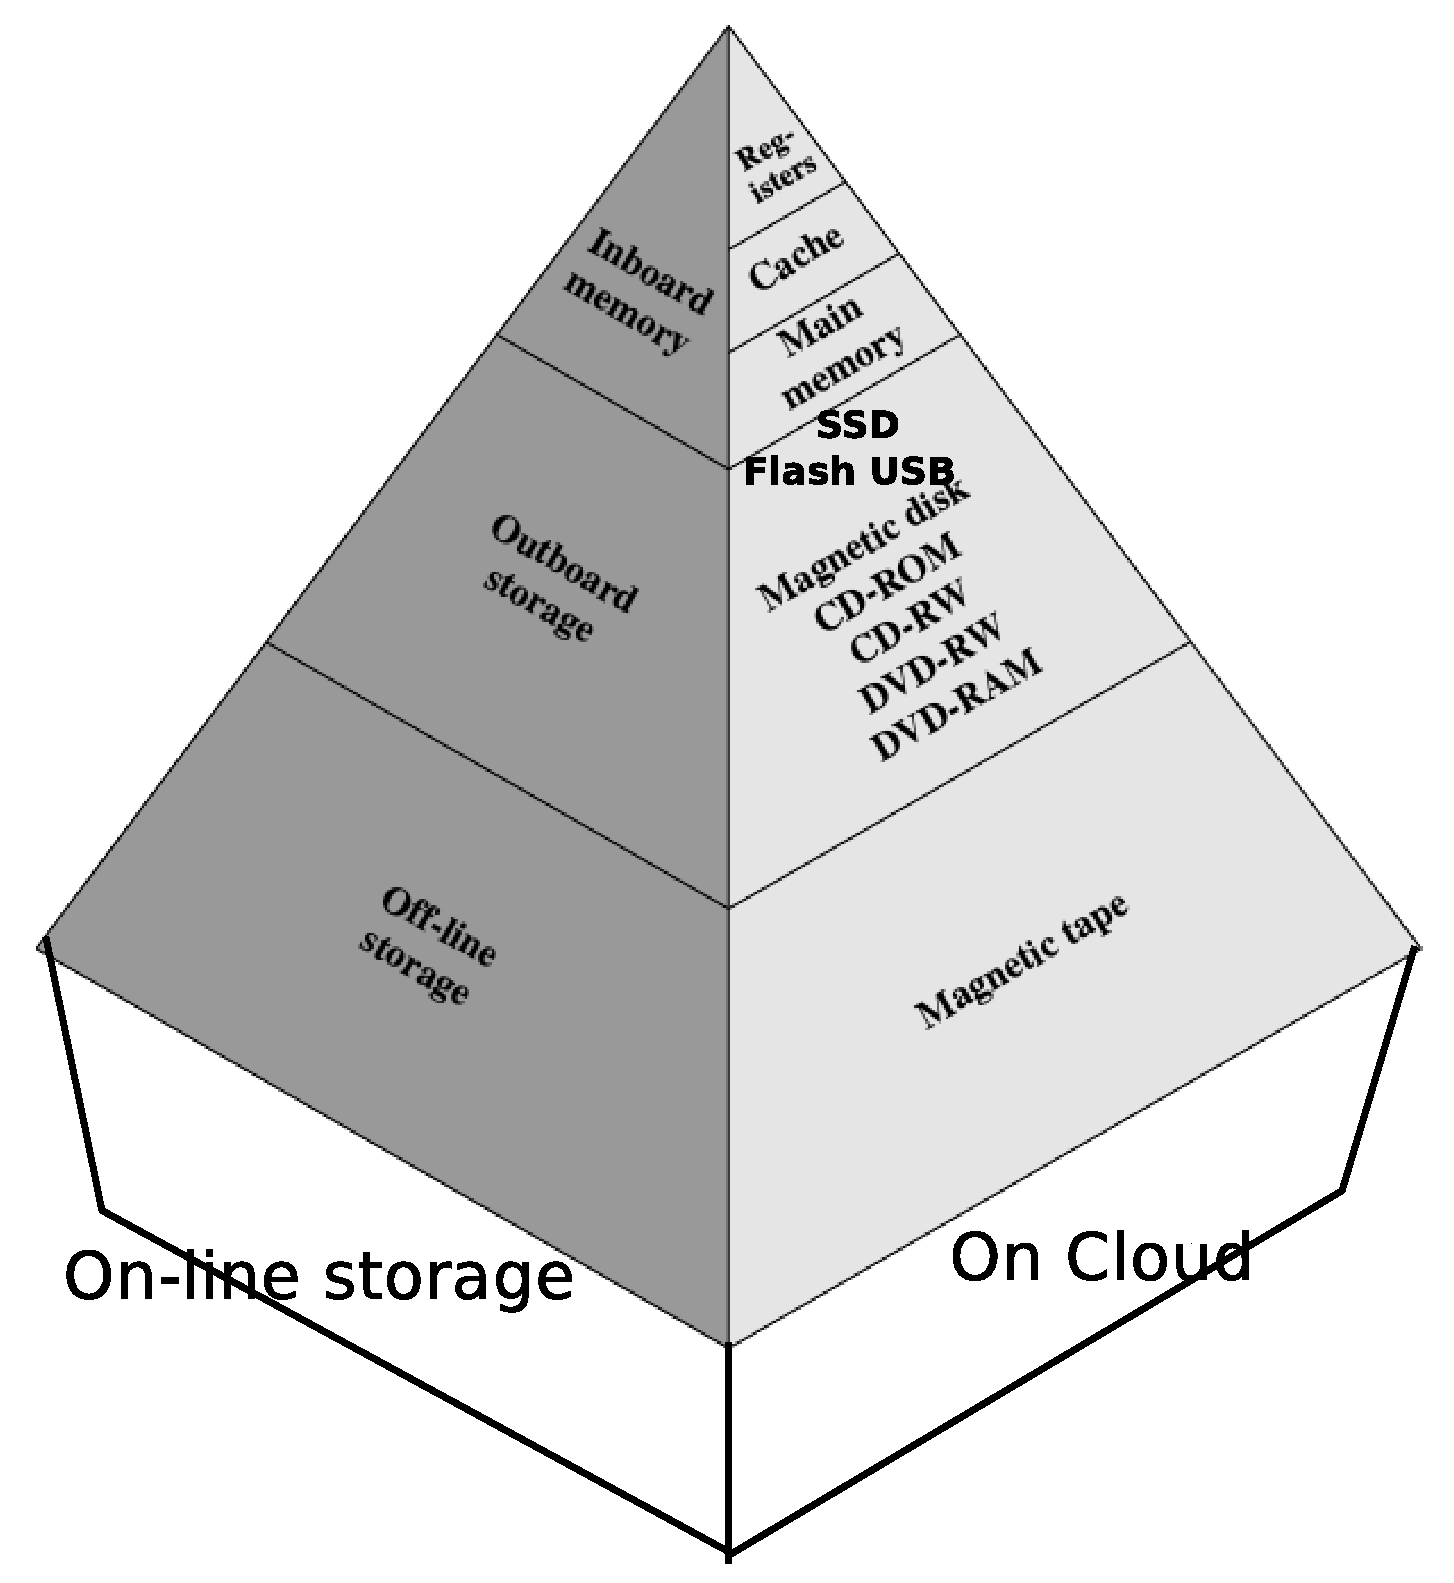
\includegraphics[width=0.6\textwidth]{images/piramidal3.eps}
\end{center}
\end{frame}
%%%%%%%%%%%%%%%%%%%%%%%%%%%%%%%%%%%%%%%%%%%%%%%%%%%%%%%%%%%%%%%%%%%%%%%%%%%%%%%%%
%%%http://www.mathcs.emory.edu/~cheung/Courses/170/Syllabus/01/intro-computer2.html
% http://rossano.pro.br/fatec/cursos/sistcomp/apostilas/assembly-1.pdf
\begin{frame}{Nível 1: Registros}
\begin{minipage}[c]{0.5\textwidth}
\begin{varblock}{Registros}
\begin{itemize}
 \item Volátil
 \item Capacidade de memoria muito pequena:{\color{red}bytes},
 \item aceso direto,
 \item velocidade muito rápida (1 ciclo para L1, 3-5ciclos para L2 e L3).
\end{itemize}
\end{varblock}
\end{minipage}
\begin{minipage}[c]{0.5\textwidth}
\includegraphics[width=1.0\textwidth]{images/register.eps}
\end{minipage}
\end{frame}

%%%%%%%%%%%%%%%%%%%%%%%%%%%%%%%%%%%%%%%%%%%%%%%%%%%%%%%%%%%%%%%%%%%%%%%%%%%%%%%%%
\begin{frame}{Nível 2: Memoria cache}
\begin{minipage}[c]{0.5\textwidth}
\begin{varblock}{Cache}
\begin{itemize}
 \item Volátil
 \item Capacidade de memoria pequena:{\color{red}$\sim25MB$},
 \item aceso aleatório aos dados,
 \item velocidade rápida.
\end{itemize}
\end{varblock}
\end{minipage}
\begin{minipage}[c]{0.5\textwidth}
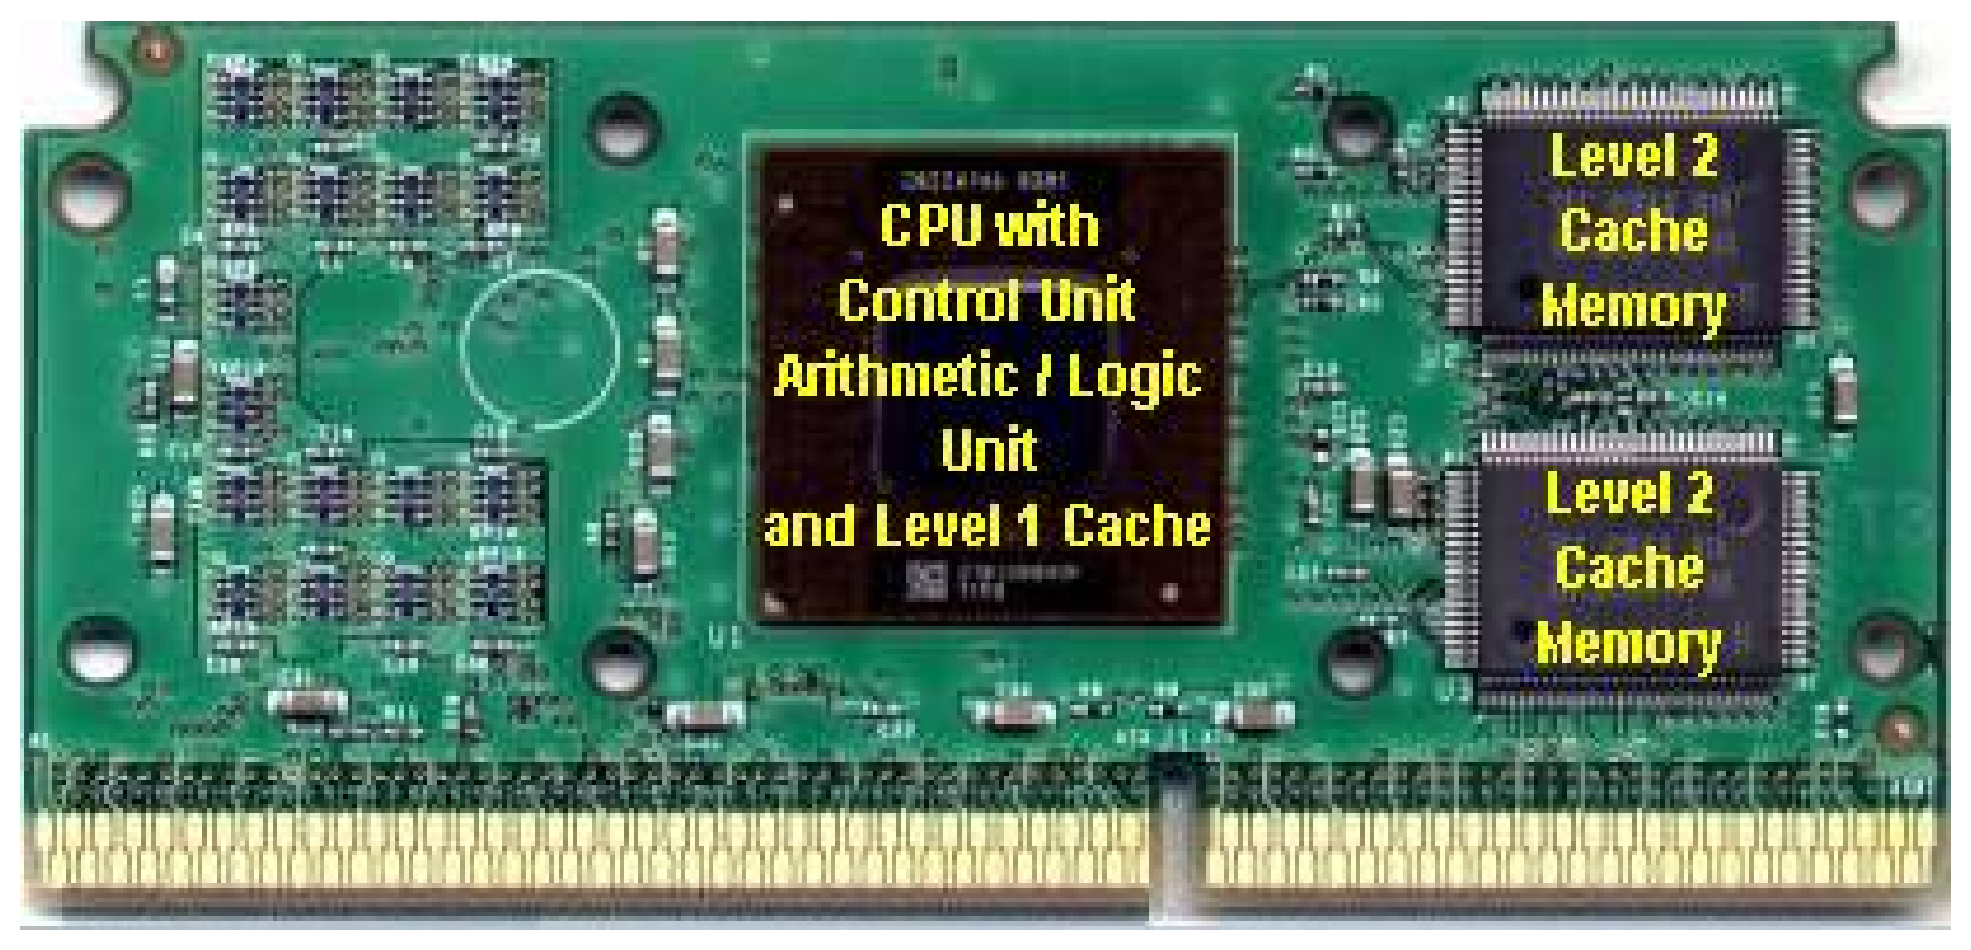
\includegraphics[width=0.9\textwidth]{images/cache.eps}
\end{minipage}
\end{frame}

%%%%%%%%%%%%%%%%%%%%%%%%%%%%%%%%%%%%%%%%%%%%%%%%%%%%%%%%%%%%%%%%%%%%%%%%%%%%%%%%%
\begin{frame}{Nível 3: Memoria principal}
\begin{minipage}[c]{0.5\textwidth}
\begin{varblock}{RAM}
\begin{itemize}
 \item Volátil
 \item Capacidade de memoria moderada:{\color{red}$\sim8GB$},
 \item aceso aleatório aos dados,
 \item velocidade moderada.
\end{itemize}
\end{varblock}
\end{minipage}
\begin{minipage}[c]{0.5\textwidth}
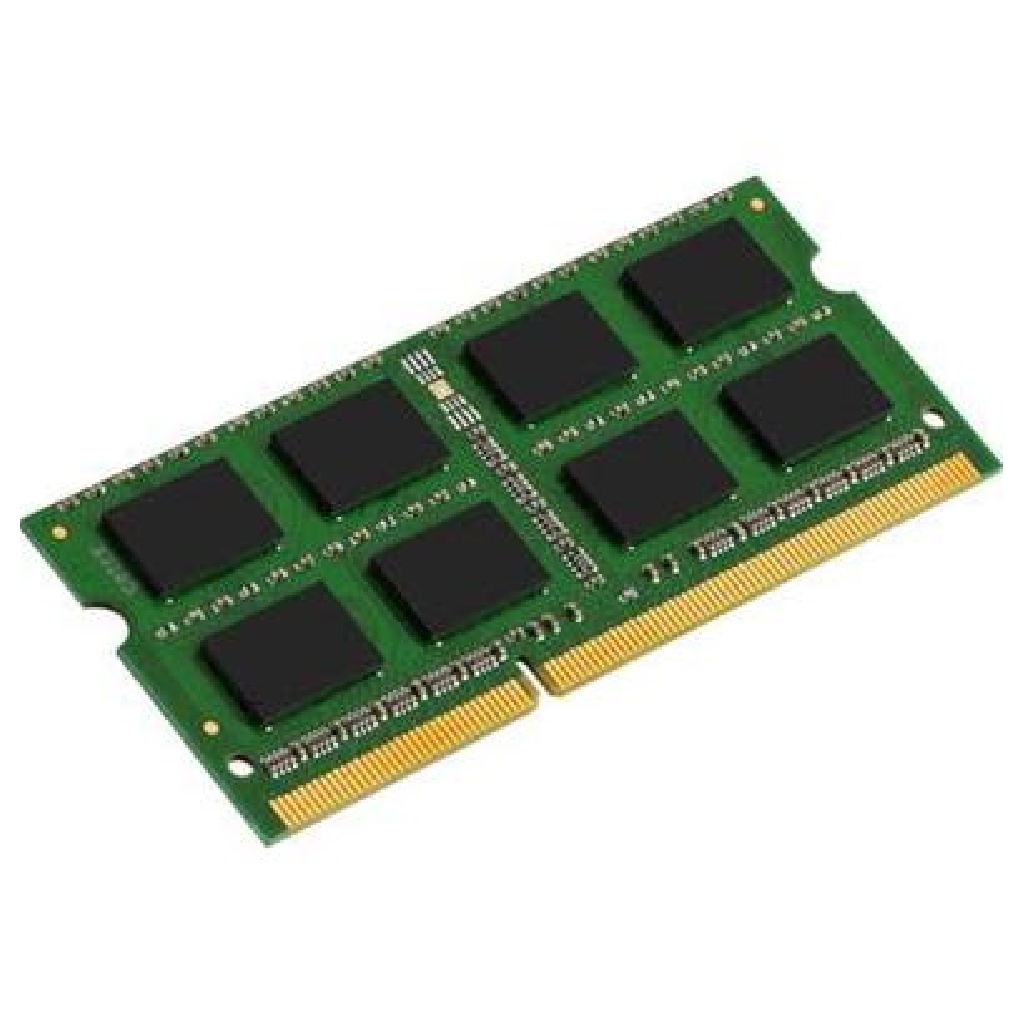
\includegraphics[width=0.9\textwidth]{images/ram.eps}
\end{minipage}
\end{frame}

%%%%%%%%%%%%%%%%%%%%%%%%%%%%%%%%%%%%%%%%%%%%%%%%%%%%%%%%%%%%%%%%%%%%%%%%%%%%%%%%%
\begin{frame}{Nível 4: SSD,USB,HD}
\begin{minipage}[c]{0.5\textwidth}
\begin{varblock}{HD,Disco rígido}
\begin{itemize}
 \item Não volátil
 \item Capacidade de memoria grande:  {\color{red}$250GB\sim2TB$},
 \item aceso aleatório ao dados,
 \item velocidade baixa.
\end{itemize}
\end{varblock}
\end{minipage}
\begin{minipage}[c]{0.5\textwidth}
\includegraphics[width=0.9\textwidth]{images/discorigido.eps}
\end{minipage}
\end{frame}

%%%%%%%%%%%%%%%%%%%%%%%%%%%%%%%%%%%%%%%%%%%%%%%%%%%%%%%%%%%%%%%%%%%%%%%%%%%%%%%%%
\begin{frame}{Nível 5: Fitas magnéticas}
\begin{minipage}[c]{0.5\textwidth}
\begin{varblock}{Sony-2014}
 Sony anunciou o 2014 que tinham desenvolvido uma fita magnética (para dados), 
 de uma densidade de  {\color{red}23 $Gbit/cm^2$}, de modo as fitas teriam
 {\color{red} 185 TB}.
\begin{itemize}
 \item Não volátil,
 \item velocidade muito baixa,
 \item dados acedidos serialmente.
\end{itemize} 
\end{varblock}
\end{minipage}
\begin{minipage}[c]{0.5\textwidth}
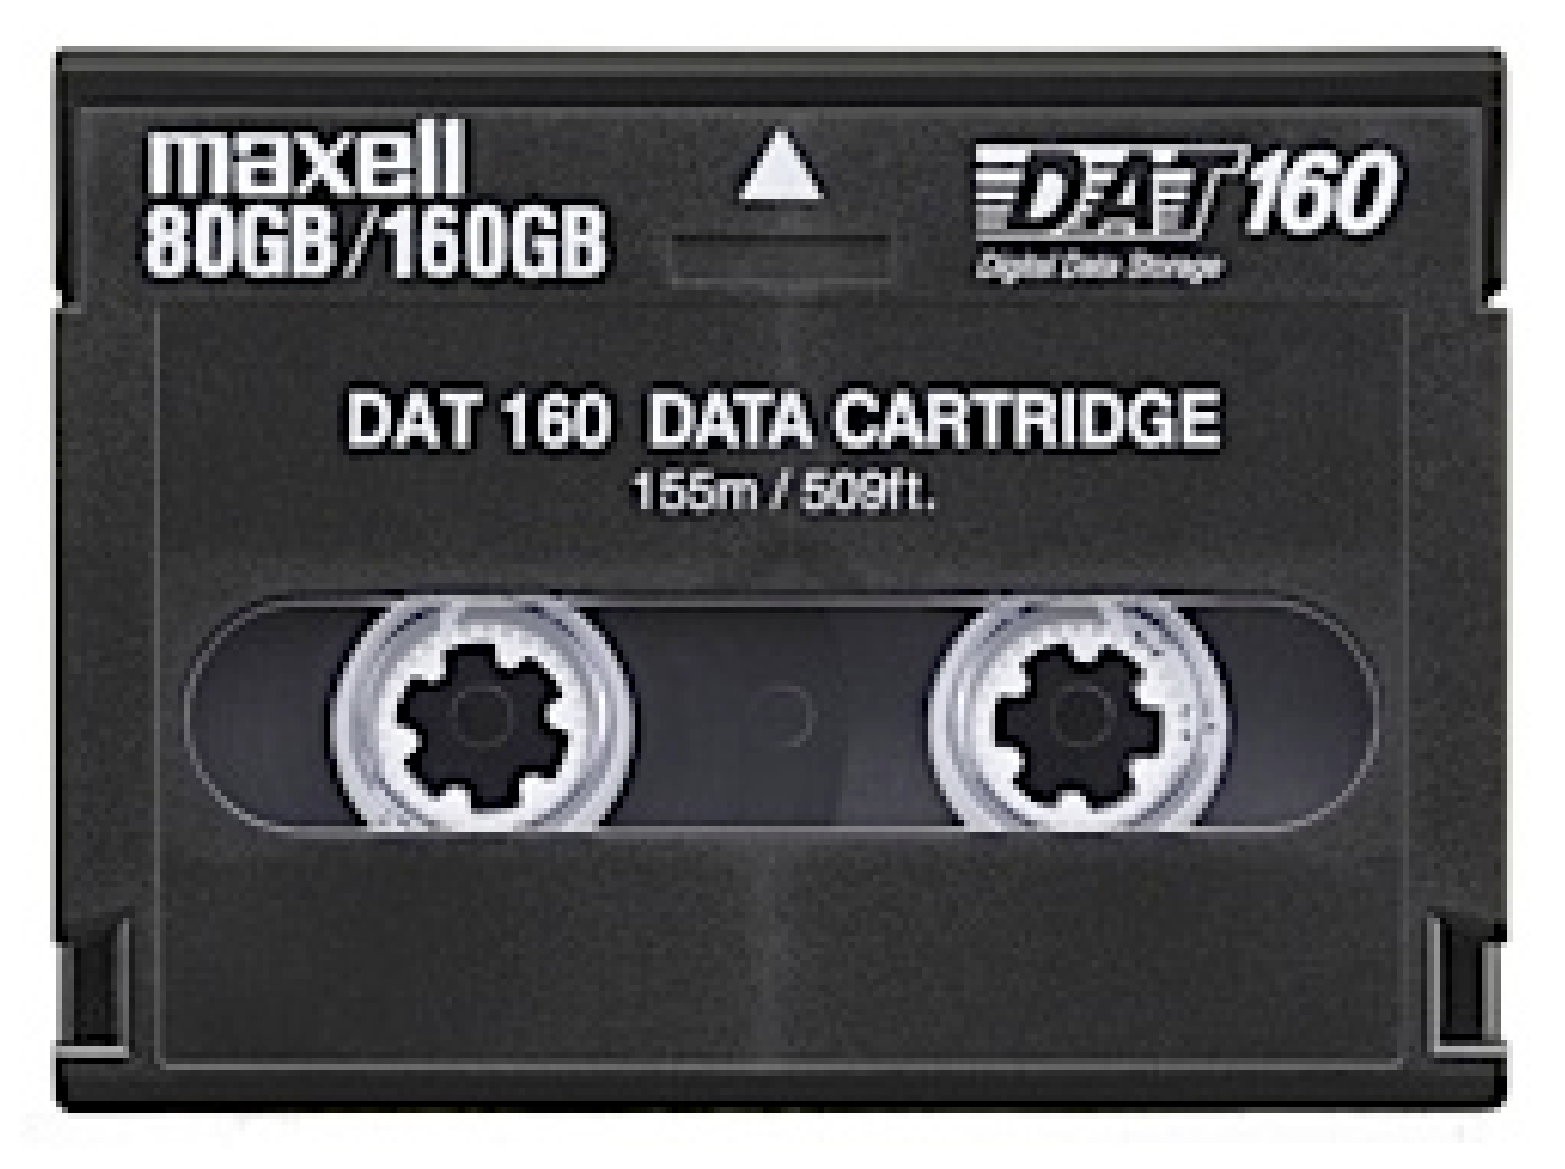
\includegraphics[width=0.9\textwidth]{images/magnetictape.eps}
\end{minipage}
\end{frame}

%%%%%%%%%%%%%%%%%%%%%%%%%%%%%%%%%%%%%%%%%%%%%%%%%%%%%%%%%%%%%%%%%%%%%%%%%%%%%%%%%
%%%%%%%%%%%%%%%%%%%%%%%%%%%%%%%%%%%%%%%%%%%%%%%%%%%%%%%%%%%%%%%%%%%%%%%%%%%%%%%%%
\section{Memoria cache}
%%%%%%%%%%%%%%%%%%%%%%%%%%%%%%%%%%%%%%%%%%%%%%%%%%%%%%%%%%%%%%%%%%%%%%%%%%%%%%%%%
\begin{frame}{Memoria cache}
\begin{center}
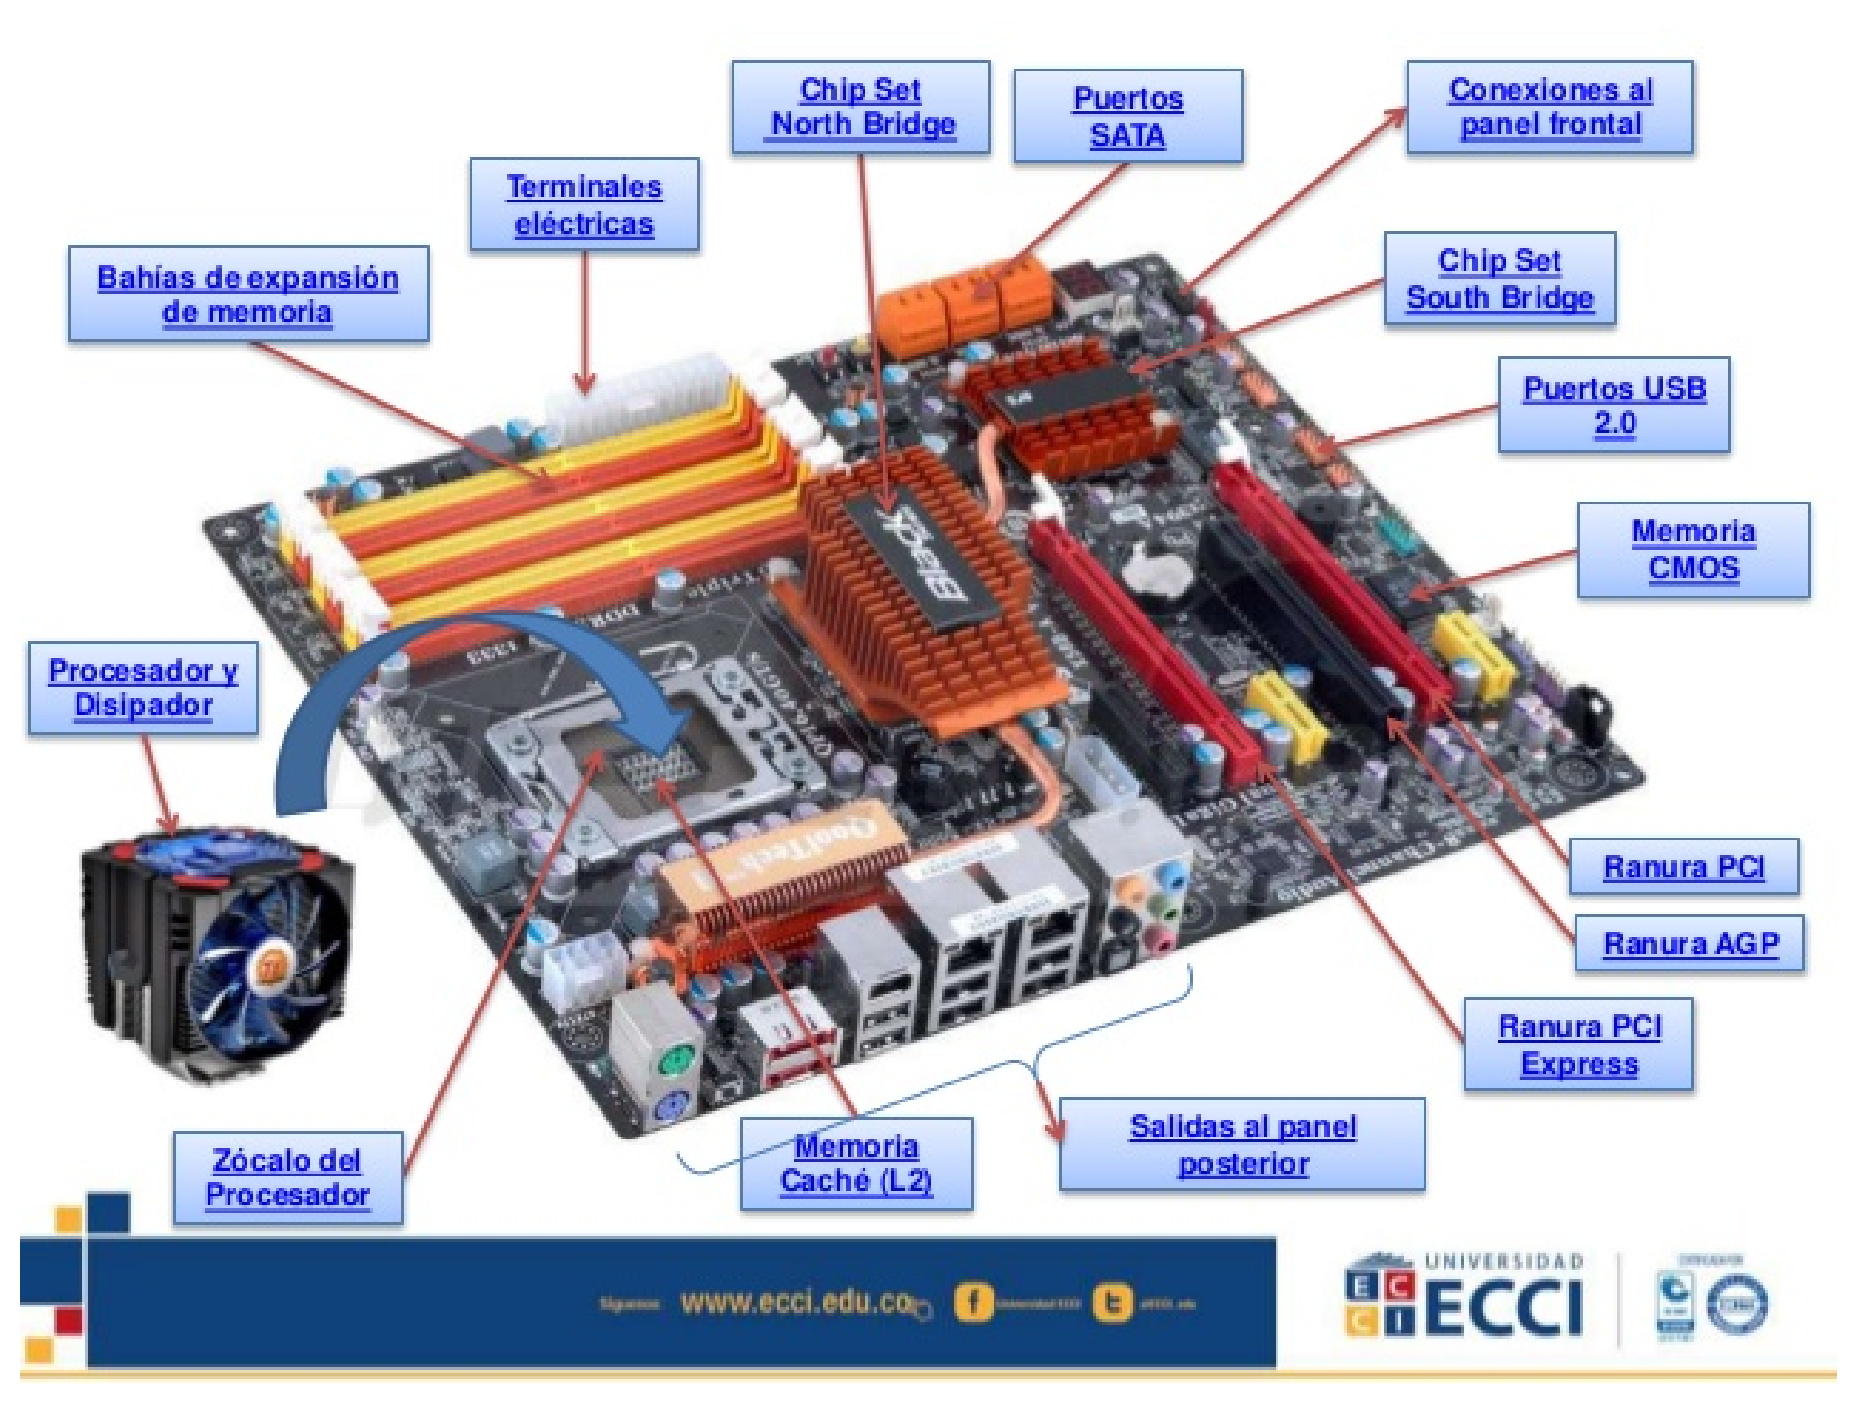
\includegraphics[width=0.8\textwidth]{images/placa1.eps}
\end{center}
\end{frame}

%%%%%%%%%%%%%%%%%%%%%%%%%%%%%%%%%%%%%%%%%%%%%%%%%%%%%%%%%%%%%%%%%%%%%%%%%%%%%%%%%
\begin{frame}{Memoria cache}
\begin{center}
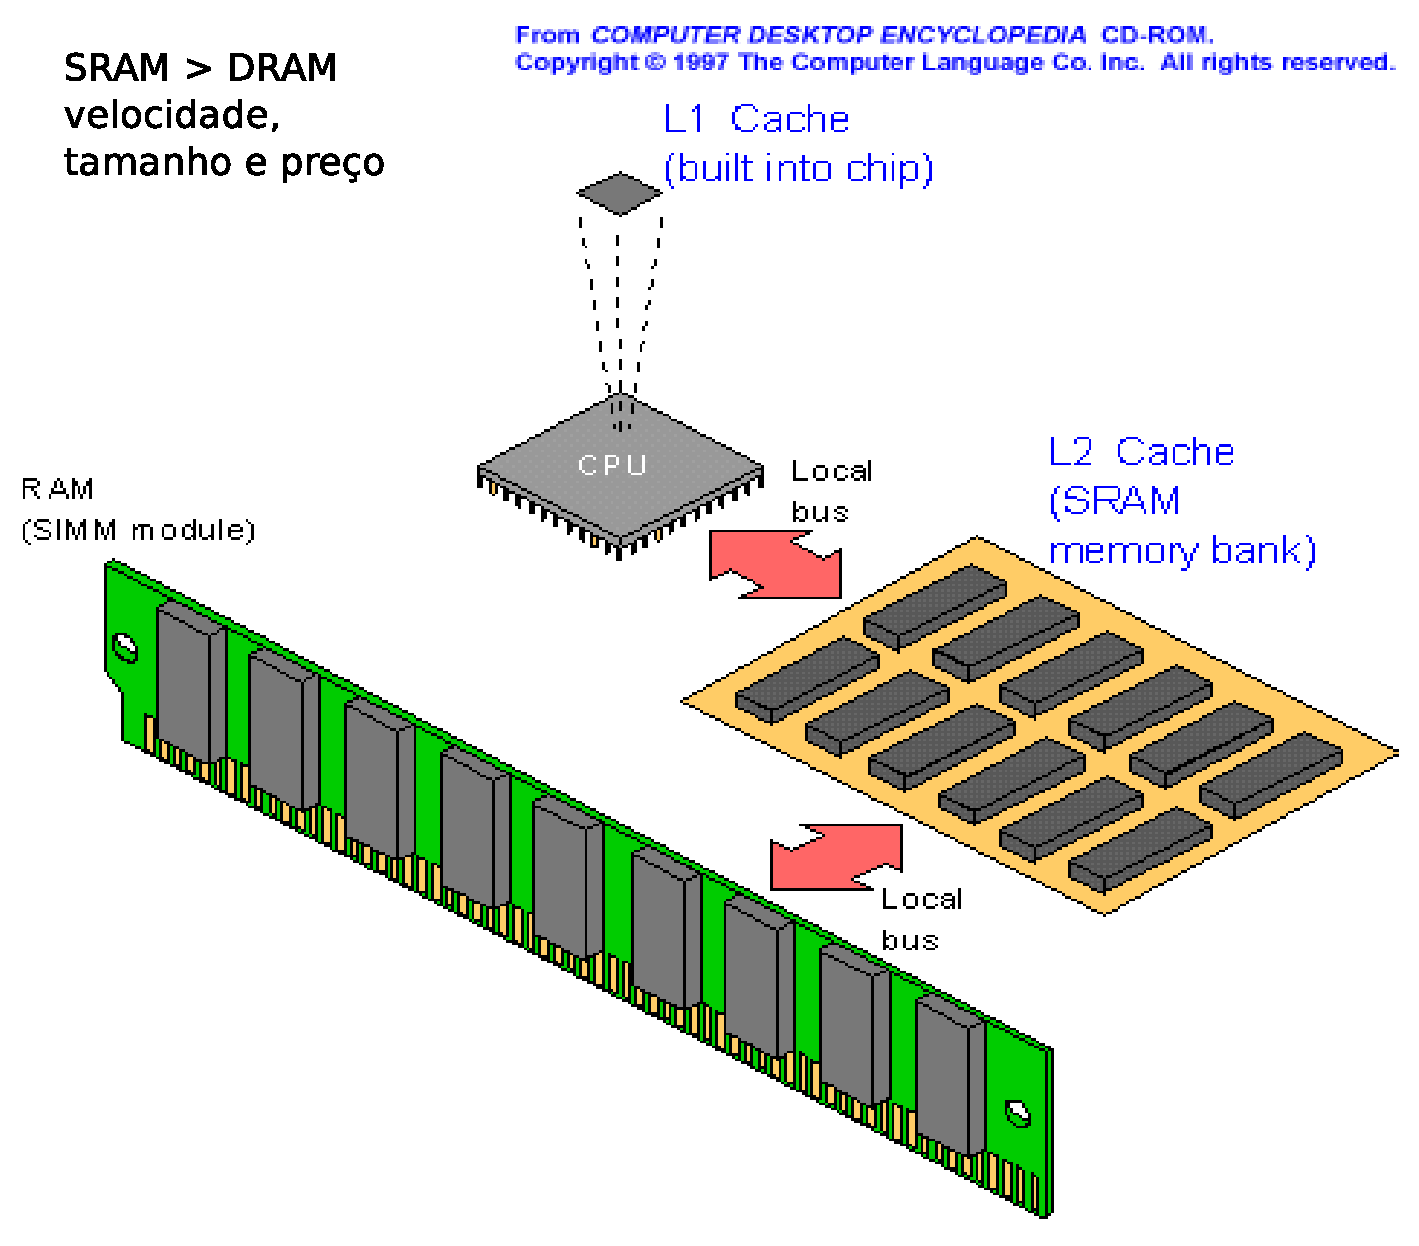
\includegraphics[width=0.6\textwidth]{images/placa2.eps}
\end{center}
\end{frame}

%%%%%%%%%%%%%%%%%%%%%%%%%%%%%%%%%%%%%%%%%%%%%%%%%%%%%%%%%%%%%%%%%%%%%%%%%%%%%%%%%
\begin{frame}{Memoria cache}
\begin{center}
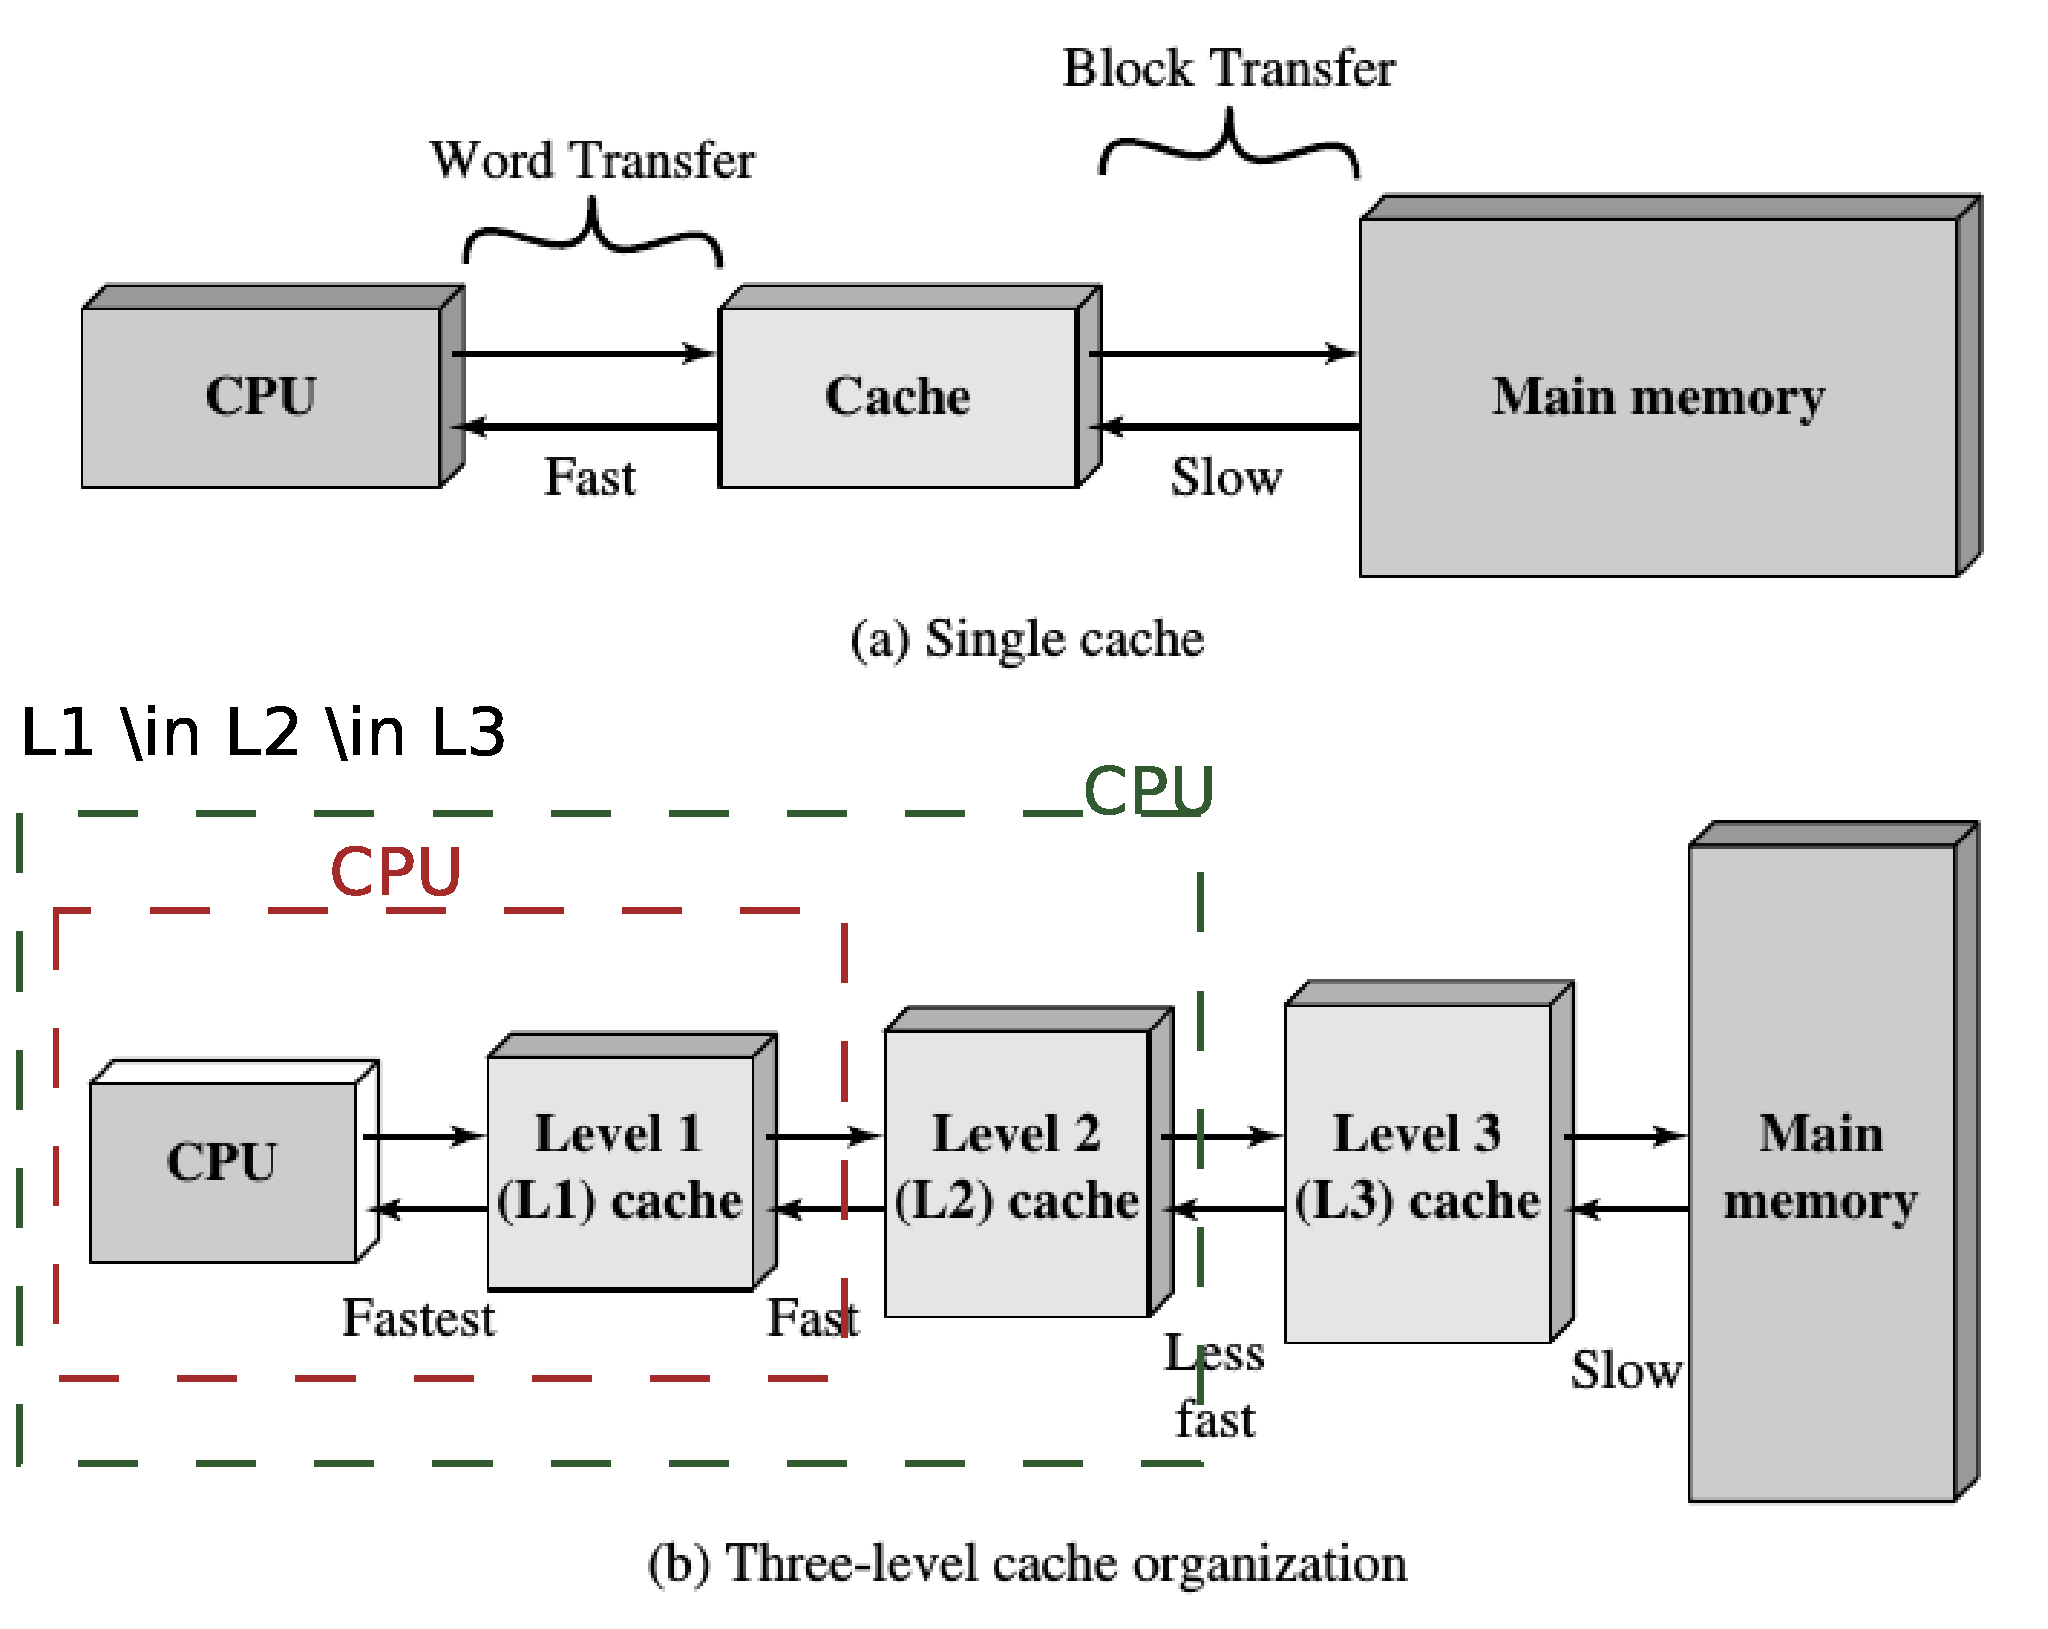
\includegraphics[width=0.6\textwidth]{images/cache1.eps}
\end{center}
\end{frame}

%%%%%%%%%%%%%%%%%%%%%%%%%%%%%%%%%%%%%%%%%%%%%%%%%%%%%%%%%%%%%%%%%%%%%%%%%%%%%%%%%
\begin{frame}{Memoria cache}
\begin{center}
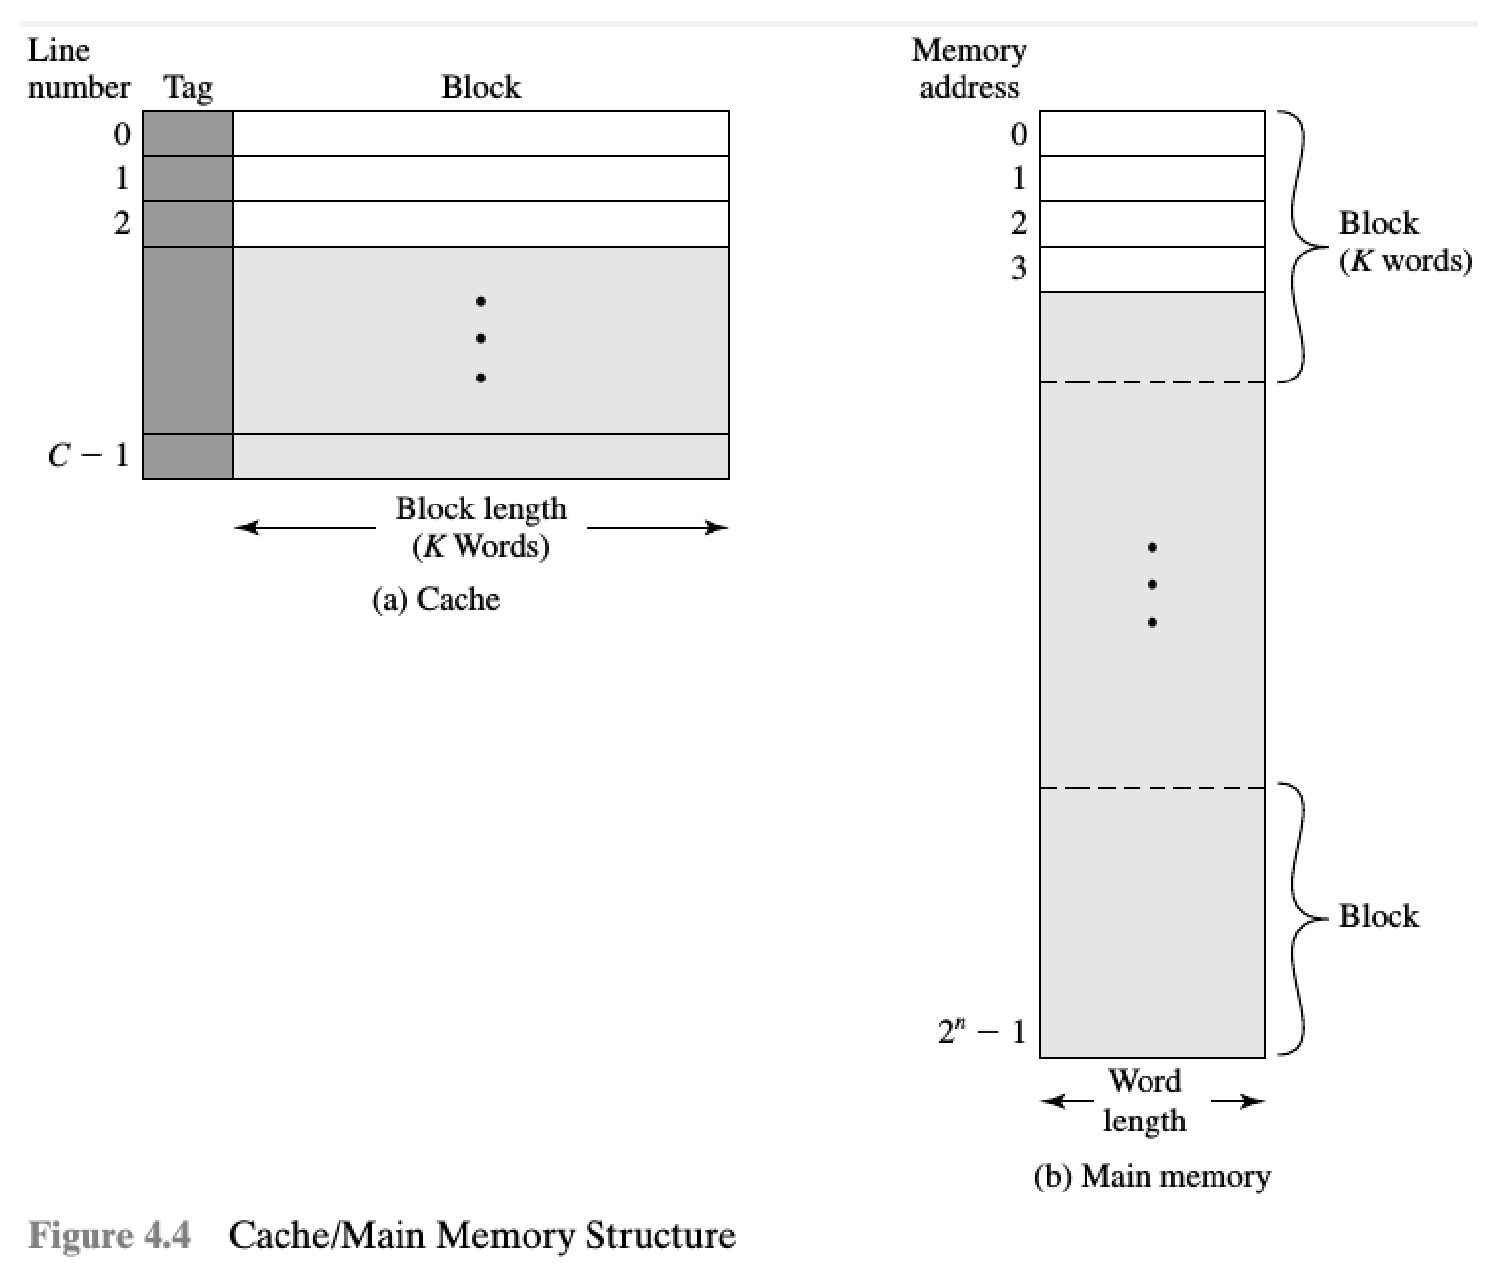
\includegraphics[width=0.6\textwidth]{images/cache2.eps}
\end{center}
\end{frame}

%https://www.youtube.com/watch?v=wrsh4D3ZF5E
%https://www.youtube.com/watch?v=FhGzGMHWkoE
%https://www.youtube.com/watch?v=Xt9KjdOdR2w
%https://www.youtube.com/watch?v=m09ZK3ngcHg
%%%%%%%%%%%%%%%%%%%%%%%%%%%%%%%%%%%%%%%%%%%%%%%%%%%%%%%%%%%%%%%%%%%%%%%%%%%%%%%%%
\begin{frame}{Memoria cache}
\begin{center}
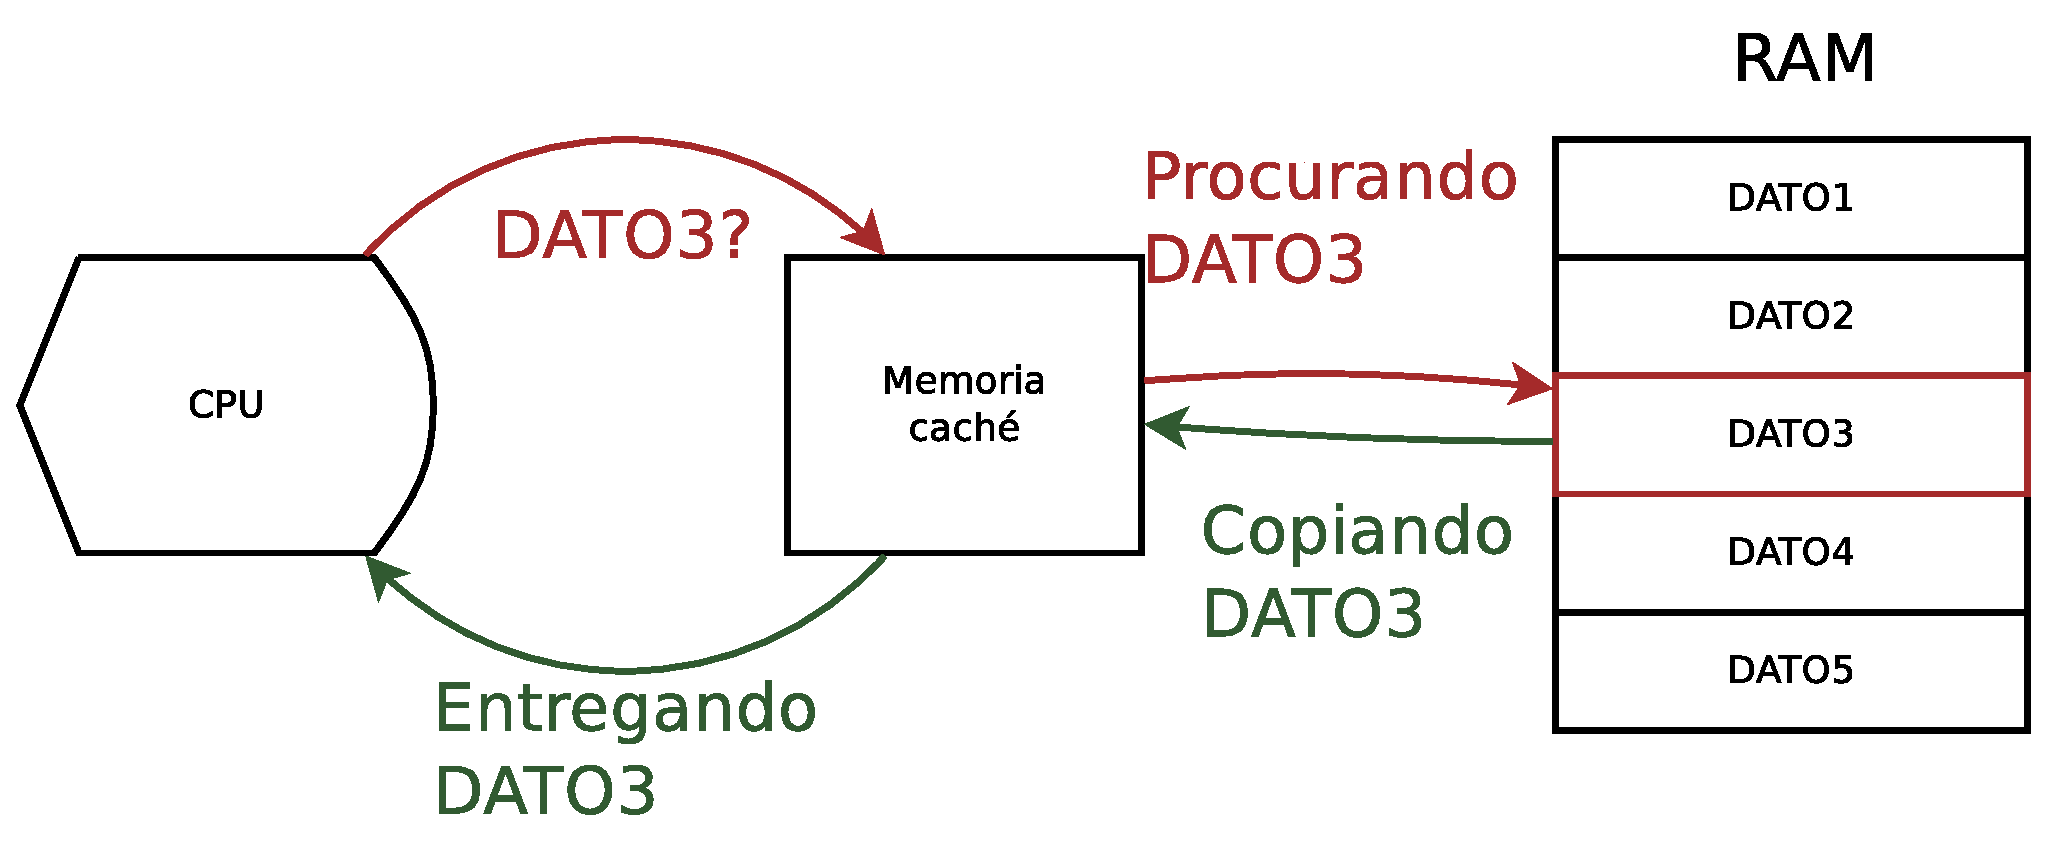
\includegraphics[width=0.8\textwidth]{images/cache3.eps}
\end{center}
\end{frame}

%%%%%%%%%%%%%%%%%%%%%%%%%%%%%%%%%%%%%%%%%%%%%%%%%%%%%%%%%%%%%%%%%%%%%%%%%%%%%%%%
\begin{frame}[allowframebreaks]
        \frametitle{References}
        \bibliographystyle{plain}
\bibliography{hierarquiamemoria}
\end{frame}



\end{document}
